\documentclass[conference]{IEEEtran}
\IEEEoverridecommandlockouts
% The preceding line is only needed to identify funding in the first footnote. If that is unneeded, please comment it out.
\usepackage{cite}
\usepackage{amsmath,amssymb,amsfonts}
\usepackage{algorithmic}
\usepackage{graphicx}
\usepackage{textcomp}
\usepackage{xcolor}
\def\BibTeX{{\rm B\kern-.05em{\sc i\kern-.025em b}\kern-.08em
    T\kern-.1667em\lower.7ex\hbox{E}\kern-.125emX}}
\begin{document}

\title{Practical Work: \\ Investigations on Remove and Retrain}

\author{\IEEEauthorblockN{1\textsuperscript{st} Viktor Maximilian Loreth}
\IEEEauthorblockA{\textit{Institute of Computational Perception} \\
\textit{Johannes Kepler University}\\
4040 Linz, Austria \\
viktor.loreth@protonmail.com}
}


\maketitle

\begin{abstract}
This report investigates the use of attribution maps in deep learning for image recognition and evaluates the effectiveness of the integrated gradient method for identifying important pixels in the MNIST dataset. In current deep learning models, it is often challenging to understand the decision-making process, making attribution maps a popular method for interpreting the importance of input features. "Remove and Retrain" offers a numerical evaluation method to evaluate attribution maps.
\end{abstract}


\section{Scientific Motivation and Goal}
Artificial neural networks have become increasingly complex in recent years, with the rise of deep learning leading to models with billions of parameters. These models have been successful in achieving state-of-the-art results on various tasks, including image recognition, natural language processing, and speech recognition. However, as these models become more complex, they also become more difficult to interpret. Creating accurate attribution maps is not a trivial task, particularly for complex models with many parameters. A well-defined attribution map highlights crucial inputs while presenting the model's response in a human-readable format. Several methods have been proposed for generating attribution maps, including gradient-based methods \cite{1_Integrated Gradient}, perturbation-based methods \cite{2_Perturbation}, and activation-based methods\cite{3_Activation}. The effectiveness of these methods can vary depending on the model architecture, the input data, and the specific task. Evaluating attribution maps is not easy due to the lack of a ground truth or reference attribution maps to compare against. Remove and Retrain is the state of the art method to evaluate attribution maps. In this report, the method is applied for Integrated Gradients on the MNIST dataset. The goal is to evaluate Integrated Gradients and reconstruct the results from the original ROAR paper.


\subsection{Trying out various methods}

At the beginning of this project, several datasets were considered for applying ROAR, including ImageNet, Food101, and MNIST. The sheer size of ImageNet\cite{4_ImageNet} presented significant computational challenges, as creating a baseline and altered datasets alone required saving a big amount of data. Additionally, generating attribution maps for this dataset and training the resNet50 \cite{5_ResNet50} model 50 times would have been too expensive considering the scope of the project.
While Food101\cite{6_Food101} offered a more manageable 50GB of data, generating attribution maps using resNET50 and training the models took too long for the available hardware. Ultimately, the MNIST dataset\cite{7_MNIST} was selected for its ease of training, ease of creating other datasets, and the potential for rapid results.

\section{Theoretical Background}
One fundamental challenge rating attribution maps is the lack of a ground truth for comparison. ROAR proposes a numerical solution to evaluate attribution maps. 
RoaR \cite{8_RoaR} works as follows:
\begin{enumerate}
	\item[1.)] Selection of the most important pixels from an attribution map\\
	An attribution map provides a mapping to the most important pixels. Those pixels are ranked based on their importance. Depending on the algorithm, different values differ on the importance. In the case of Integrated Gradient, the pixels with the highest absolute values are considered the most important.
	\item[2.)] Replacement of x\% of the pixels with the mean value\\
	In the Roar algorithm, 0.1, 0.3, 0.5, 0.7 or 0.9 \% of the most important pixels are identified and replaced by the mean value. Both the training and the testing data undergo this process.
	\item[3.)] Retraining the model using the modified dataset\\
	To ensure the consistency of the model, retraining is necessary. Afterwards, the model is evaluated using several seed runs on the test set. The same split should be used for all runs.
	This is crucial, because the training data and the test data must be drawn from the same distribution. Without retraining the model this property is ignored.
	\item[4.)] Comparison of the attribution map with a random baseline \\
	For each training setup, respectively with 0.1, 0.3, 0.5, 0.7 or 0.9 \% pixels replaced, a random baseline is considered. The random baseline also replaces the same percentage of pixels. The random baseline is expected to perform worse than a sophisticated method.
	\item[5.)] Evaluation \\
	An attribution method is deemed effective, if it consistently outperforms the random baseline across various setups.
\end{enumerate}


\section{Training}
\subsection{Training the model}
The model used in this report is a simple convolution neural network architecture consisting of two convolution layers, two pooling layers, and three linear layers. The model was trained for ten epochs with a learning rate of 1e-3 and a SGD optimizer with a momentum term of 0.9. The batch size was 64. Across five separate runs, the model achieved an average accuracy of 97.4\% with a standard deviation of 0.4\% on the test data.

\subsection{Data set preparation and Splitting}\label{AA}

The MNIST data set consists of 10 classes and 70.000 different images. It was chosen, because it is easy to evaluate the effectiveness of integrated gradients and ROAR: a) The importance of the pixels is clear from a human perspective. b) The model required to achieve a solid performance is very modest and speeds up the retraining. c) The information loss in retraining is clearly see able in the pictures.\\ Furthermore, it is a small, usable data set. The images are 28x28 pixels big and one pixel has a value ranging from [0,1] in the gray-scale.
The data set used in this report was normalized using the mean and standard deviation, and was split using the PyTorch library's default splitting method (60.000 images for the training data, 10.000 images for the test data). The training data was shuffled randomly using the inbuilt functions.  Cross entropy loss was selected for training runs. The same data set split was used for all training runs to ensure consistency in the results.


\subsection{Example of the new dataset}

In Figure 1 the difference between Integrated Gradients and the Random Baseline is visible. In the first row the random baseline is visible, in the second row Integrated Gradients is shown. [0.1,0.3,0.5,0.7,0.9\%] of the pixels are blacked out (left to right).

\begin{figure}[h]
	\centering
	\includegraphics[width=0.5\textwidth]{figs/IGvsRandom.png}
	\caption{Integrated Gradients and Random Baseline Comparison}
	\label{fig:igvsR}
\end{figure}

 As visible by human intuition, Integrated Gradients is appearing to perform better over all thresholds. The model is expected to perform worse following retraining.

\subsection{Retraining upon the new datasets}

To ensure that the model learns consistently, the same split and learning parameters were utilized as in the standard case to retrain the model on the new data set. An untrained network was created and then retrained for each training run. In order to validate the results and minimize the impact of random seed initialization, the training was performed with 5 different seeds and 5 models were created. In the Appendix the exact results can be found. 

\subsection{Advantages and Disadvantages of the setup}

Because of the small size of the data set and the limited amount of classes, training a model is fast and effective. \\
One disadvantage is the limited generalization of this setup for other datasets and models. The majority of use cases primarily involve working with images in the RGB color space, utilizing deep learning models that are often more complex, and dealing with a larger number of distinct classes. Furthermore, the pixels itself are blurred on their importance. In RGB images 3 channels are combined, which make attribution maps more difficult to compute and understand. 


\section{Results}

To compare the effectiveness of the attribution map, it was compared to a random baseline, which masked x\% of the pixels randomly. The expected result is a consistently higher accuracy in the random baseline vs the Integrated Gradients. This should show in any \% of pixels blocked out.
If an attribution maps blocks out sufficiently enough pixels which are informative for the model, then the accuracy should decline. The random baseline should, in comparison, find less important pixels more frequently and therefore have a higher accuracy.


\subsection{Interpretation of results}

In Fig 2 it is shown that Integrated Gradients learns significantly worse than the Random Baseline and at 90\% of the pixels removed the performance is as good as a random guess: 10\%. This implies that Integrated Gradient is a better attribution map than the random baseline.


\begin{figure}[h]
	\centering
	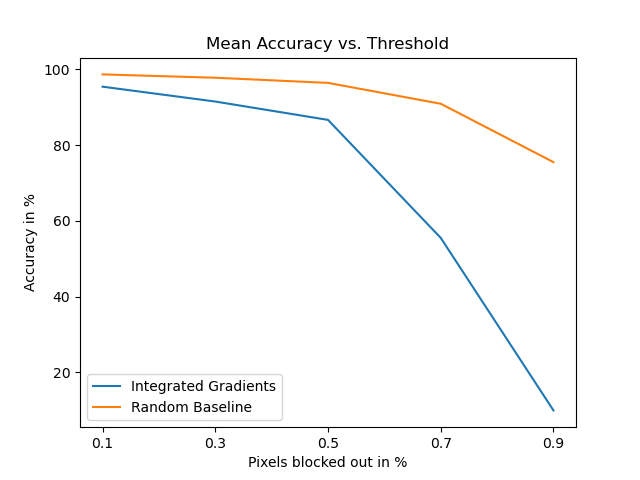
\includegraphics[width=0.5\textwidth]{figs/mean_accuracy_vs_threshold.png}
	\caption{Mean Accuracy vs Threshold}
	\label{fig:mean_accuracy}
\end{figure}


\newpage

The increasing standard deviation (Table 1) indicates that the model can no longer learn reliably, suggesting that it is identifying arbitrary new structures in the images that it interprets incorrectly. While adjusting the learning parameters may improve scores, it is clear that accuracy is lower than at other thresholds.

\begin{table}[ht]
	\centering
	\begin{tabular}{|c|c|c|c|c|c|}
		\hline
		Pixels removed & 10\% & 30\% & 50\% & 70\% & 90\% \\
		\hline
		Integrated Gradient & 0.44\% & 0.83\% & 2.10\% & 31.64\% & 0\% \\
		Random Baseline  & 0.42\% & 0.28\% & 0.39\% & 0.58\% & 0.65\% \\
		\hline	
	\end{tabular} \newline
	
	\caption{Standard deviation of mean accuracy over 5 Training runs}
	\label{tab:std_deviation}
\end{table}

In the Appendix the precision of the models are presented. For the integrated gradient method there exist a higher standard deviation and a lower precision, which means that the models are not able to learn reliably anymore. On the other hand, the random baseline still has a very good performance even after removing 90\% of the pixels.


\subsection{Are the results meaningful?}

Due to the fact, that the accuracy declines so slowly, it is unclear if the results given are really meaningful. Furthermore, there is no real threshold. To provide a theoretical explanation for the implications of removing input dimensions on the resulting accuracy, the following factors should be considered \cite{8_RoaR}:


\begin{enumerate}
	\item[1.)] Input dimensions are removed and the accuracy drops:
	
	The removed input were informative for the model and their absence reduces the ability of the model to identify the right class.
	
	\item[2.)] We remove inputs and the accuracy does not drop.
	\\
	(a)  It is possible that the removed input dimensions were not important for the model's decision-making process. The attribution map failed to identify important features, such as pixels on the image borders in the case of MNIST.
	(b) The input could be redundant and the information be reconstructed using other available inputs. In the scenario where nine white surrounding pixels are white and one blurred pixel is in the middle, the network still recognizes the blurred features, even if it is removed from the input.
\end{enumerate}

The ROAR method effectively demonstrates the better performance of Integrated Gradients as an attribution map against a random baseline on the MNIST dataset. Contrary to the results in \cite{8_RoaR}, Integrated Gradient is successfully finding meaningful pixels. This may be attributed to the large size of the ResNET50 model, but more investigation is needed to make a proper statement. 


\begin{thebibliography}{00}
	
\bibitem{1_Integrated Gradient} M. Sundararajan, A. Taly, and Q. Yan, "Axiomatic Attribution for Deep Networks," in \textit{Proceedings of the 34th International Conference on Machine Learning, {ICML} 2017, Sydney, NSW, Australia, 6-11 August 2017}, pp. 3319-3328, 2017. Available: http://proceedings.mlr.press/v70/sundararajan17a.html
	
\bibitem{2_Perturbation} 
Ribeiro, M. T., Singh, S., Guestrin C., "Why Should {I} Trust You?": Explaining the Predictions of Any Classifier", Proceedings of the 22nd {ACM} {SIGKDD} International Conference on Knowledge Discovery and Data Mining, San Francisco, CA, USA, August
13-17, 2016, Available: https://doi.org/10.1145/2939672.2939778

\bibitem{3_Activation} 
Ramprasaath R. Selvaraju, Michael Cogswell, Abhishek Das, Ramakrishna Vedantam, Devi Parikh and Dhruv Batr, "Grad-CAM: Visual Explanations from Deep Networks via Gradient-Based Localization", Int. J. Comput. Vis., Vol: 128, 336--359, 2020, Available: https://doi.org/10.1007/s11263-019-01228-7

\bibitem{4_ImageNet} J. Deng, W. Dong, R. Socher, L.-J. Li, K. Li, and L. Fei-Fei, "ImageNet: A large-scale hierarchical image database," in \textit{2009 IEEE Computer Society Conference on Computer Vision and Pattern Recognition (CVPR 2009), 20-25 June 2009, Miami, Florida, USA}, pp. 248-255, 2009. doi: 10.1109/CVPR.2009.5206848. Available: https://doi.org/10.1109/CVPR.2009.5206848

\bibitem{5_ResNet50} K. He, X. Zhang, S. Ren, and J. Sun, "Deep Residual Learning for Image Recognition," in \textit{2016 IEEE Conference on Computer Vision and Pattern Recognition, CVPR 2016, Las Vegas, NV, USA, June 27-30, 2016}, pp. 770-778, 2016. doi: 10.1109/CVPR.2016.90. Available: https://doi.org/10.1109/CVPR.2016.90

\bibitem{6_Food101} L. Bossard, M. Guillaumin, and L. Van Gool, "Food-101 - Mining Discriminative Components with Random Forests," in \textit{Computer Vision - ECCV 2014 - 13th European Conference, Zurich, Switzerland, September 6-12, 2014, Proceedings, Part VI}, pp. 446-461, 2014. doi: 10.1007/978-3-319-10599-4\_29. Available: https://doi.org/10.1007/978-3-319-10599-4\_29



\bibitem{7_MNIST} 
L. Deng, "The {MNIST} Database of Handwritten Digit Images for Machine Learning Research [Best of the Web]," \textit{IEEE Signal Process. Mag.}, vol. 29, no. 6, pp. 141-142, 2012. doi: 10.1109/MSP.2012.2211477. Available: https://doi.org/10.1109/MSP.2012.2211477
	
\bibitem{8_RoaR} S. Hooker, D. Erhan, P.-J. Kindermans, and B. Kim, "A Benchmark for Interpretability Methods in Deep Neural Networks," in \textit{Advances in Neural Information Processing Systems 32: Annual Conference on Neural Information Processing Systems 2019, NeurIPS 2019, December 8-14, 2019, Vancouver, BC, Canada}, H. M. Wallach et al. (Eds.), pp. 9734-9745, 2019. Available: https://proceedings.neurips.cc/paper/2019/hash/fe4b8556000d0f0cae99d\\aa5c5c5a410-Abstract.html
% To reformat












\end{thebibliography}
\onecolumn
\newpage



\section{Appendix}
\centering
Precision and standard deviation of the retrained models per threshold.

\begin{table}[h]
	\centering
	\begin{tabular}{|c|c|c|c|c|c|c|c|c|c|c|}
		\hline
		
		Pixels removed & 0 & 1 & 2 & 3 & 4 & 5 & 6 & 7 & 8 & 9 \\
		\hline
		10\%& 97.2 & 95.4 & 96.2 & 94.6 & 95.6 & 97.2 & 98.4 & 96.2 & 92.8 & 90.4 \\
		std & 0.98 & 0.80 & 0.98 & 1.36 & 1.62 & 2.04 & 1.50 & 2.71 & 1.83 & 3.61 \\
		\hline
		30\% &  94.6 & 95.4 & 92.4 & 87.0 & 86.2 & 91.4 & 96.2 & 92.4 & 87.8 & 91.4 \\
		std & 2.06 & 1.74 & 2.94 & 6.26 & 2.79 & 3.26 & 0.98 & 2.50 & 2.56 & 2.94 \\
		\hline
		50\% &93.8 & 89.6 & 82.6 & 85.2 & 79.0 & 92.4 & 94.2 & 88.8 & 73.8 & 87.0  \\
		std & 2.64 & 4.03 & 4.84 & 5.42 & 1.90 & 4.13 & 2.14 & 3.60 & 5.74 & 1.79 \\
		\hline
		70\% & 74.2 & 88.0 & 52.0 & 59.4 & 35.6 & 50.0 & 55.2 & 55.8 & 41.4 & 43.6  \\
		std & 37.1 & 7.5 & 38.6 & 38.8 & 30.1 & 40.9 & 45.1 & 36.0 & 34.5 & 35.6 \\
		\hline
		90\% & 0.00 & 100.00 & 0.00 & 0.00 & 0.00 & 0.00 & 0.00 & 0.00 & 0.00 & 0.00  \\
		std & 0.00 & 0.00 & 0.00 & 0.00 & 0.00 & 0.00 & 0.00 & 0.00 & 0.00 & 0.00 \\
		\hline
	\end{tabular} \newline
	
	\caption{Class Precision and Std deviation (values in \%) Integrated Gradient}
	\label{tab:sclass_precision_ig}
\end{table}



\begin{table}[h]
	\centering
	\begin{tabular}{|c|c|c|c|c|c|c|c|c|c|c|}
		\hline
		
		Pixels removed & 0 & 1 & 2 & 3 & 4 & 5 & 6 & 7 & 8 & 9 \\
		\hline
		10\%& 100.0 & 100.0 & 97.2 & 100.0 & 98.4 & 98.4 & 98.8 & 98.0 & 96.8 & 98.8 \\
		std & 0.0 & 0.0 & 0.98 & 0.0 & 0.8 & 0.8 & 0.98 & 1.26 & 1.47 & 1.60 \\ 
		\hline
		30\% &  98.4 & 99.6 & 98.0 & 98.8 & 95.2 & 98.0 & 97.6 & 97.6 & 98.4 & 96.0 \\
		std & 0.80 & 0.80 & 1.26 & 1.60 & 1.17 & 1.79 & 0.80 & 1.50 & 0.80 & 1.90 \\
		\hline
		50\% &100.0 & 96.4 & 95.0 & 96.6 & 94.2 & 97.2 & 99.2 & 95.6 & 94.8 & 95.0 \\
		std & 0.00 & 1.20 & 1.55 & 1.96 & 2.64 & 1.60 & 1.60 & 0.49 & 1.47 & 1.10 \\
		\hline
		70\% & 95.8 & 95.4 & 92.2 & 86.0 & 90.0 & 91.8 & 94.0 & 93.8 & 85.2 & 84.8 \\
		std & 1.60 & 0.80 & 3.66 & 3.95 & 2.76 & 2.32 & 1.79 & 1.47 & 3.06 & 4.87 \\
		\hline
		90\% & 87.4 & 89.2 & 85.6 & 67.6 & 56.8 & 71.4 & 85.2 & 79.8 & 68.8 & 63.2  \\
		std & 1.96 & 0.98 & 4.32 & 4.36 & 8.80 & 5.31 & 1.17 & 2.86 & 4.96 & 6.97 \\
		\hline
	\end{tabular} \newline
	
	\caption{Class Precision and Std deviation (values in \%) Random Baseline}
	\label{tab:sclass_accuracy_random}
\end{table}


% restore original margins
\vspace{12pt}
\color{red}

\end{document}
